\chapter{SFC Implementation}
\label{chap:impl}

\newcommand{\enchainer}{\texttt{Enchainer}}
\newcommand{\vnf}{\texttt{VNF}}
\newcommand{\vnfs}{\texttt{VNFs}}
\newcommand{\dispatcher}{\texttt{Dispatcher}}

In this chapter there is described the implementation of the solution that we
proposed for the SFC system. Also the experimental implementation that allow us
to reach the final solution are discussed and why they where abandoned.

\section{Kubernetes Pods and our implementation}
\todo{Describing pods}

\section{How to reach virtual functions}
The first issue to overcome in our implementation was how to make possible to
reach Pods inside Kubernetes without specifying the IP of the machine on the top
of which they are running. In fact, enabling that possibility would allowed us
to create a flexible and scalable solution. In fact, decoupling Pods to physical
machine let our proposal to be independent on the underlying infrastructure: the
addition or the removal of hosts would be transparent for the code developed,
demanding to Kubernetes the task of manage the change in computational and
storage resources. Kubernetes services \todo{add reference} allowed us to
overcome the problem. \todo{add Kubernetes services explanation}

\subsection{Kubernetes Services}
A Kubernetes service is an abstraction that defines a set of Pods and policies
to access them. Pods referenced by a certain Service are usually selected with a
\emph{Label Selector}. In general these labels, added to Pod specifications,
does not provide uniqueness but identify a set of objects.
In the snipped~\ref{chap:impl:lst:srv} there is an example of Service
definition.The service create will be called \texttt{my-service} and targets TCP
port 9376 on any Pods labelled with the selector \texttt{app=MyApp}. Kubernetes
will assign to the Service an IP address (also called \emph{clusterIP}). 
\texttt{port} filed in the definition is the port on which the Service can be
reached, instead \texttt{targetPort} is the port on which traffic will be
redirected on Pods. It can be either a valid port number or a string that
identify port name of backend Pods, allowing more flexibility to Pod and Service
creation. Supported protocols are TCP, UDP and SCTP. \texttt{kube-proxy} is
accountable for implementing virtual IP for Services (other than Services with
type \texttt{ExternalName}). 

\begin{lstlisting}[caption={Example of Service definition},
                   captionpos=b, language=yaml, label=chap:impl:lst:srv]
kind: Service
apiVersion: v1
metadata:
  name: my-service
spec:
  selector:
    app: MyApp
  ports:
  - protocol: TCP
    port: 80
    targetPort: 9376
\end{lstlisting}

For Service discovery, there were \emph{environment variables} and \emph{DNS}.
To Pods running on a certain Node \texttt{kubelet} add a set of variables for
each Services, that can be used for referencing to it. In the former technique,
to discover services, instead, are used the DNS server cluster add-on. It
watches Kubernetes API to be aware if new Services are created to add DNS
records for them. In this way all Pods are able to do Service name resolution
automatically. Services types can be:
\begin{description}
\item[ClusterIP:] to expose services only within the cluster, it is the default
value;
\item[NodePort:] to expose the service on a static port. Outside the cluster is
reachable by requesting \verb!<NodeIP>:<NodePort>!
\item[LoadBalancer:] to expose a service externally, using a cloud provider
load balancer;
\item[ExternalName:] to expose a service with the name expressed in the 
\texttt{externalName}.
\end{description}

All services that we used belong to \texttt{NodePort} category. This choice was
made for a twofold reason. First is the sake of simplicity: binding services to
a predefined port is easy to concatenate services and identify them by port.
\texttt{NodePort} type is not suitable to expose services to the outside world,
as instead \texttt{ExternalName}. However it requires the registration of a
domain name. In a production ready platform or in a more advanced testbed,
alternative type of services can be used.

Taking advantage of that, we decided that all components of our solution that
will be deployed on Kubernetes will be exposed by a service. In this manner, to
reach a defined component in our solution it is possible to only specify the
name of the service and the port to which it is bound. Kubernetes is in charge
to decide which Pod to reach (if more replicas of the same function are
available) in the pool labelled to belong to the same service, resolving the
location on which it is deployed.

\section{First review}
\begin{figure}
  \centering
  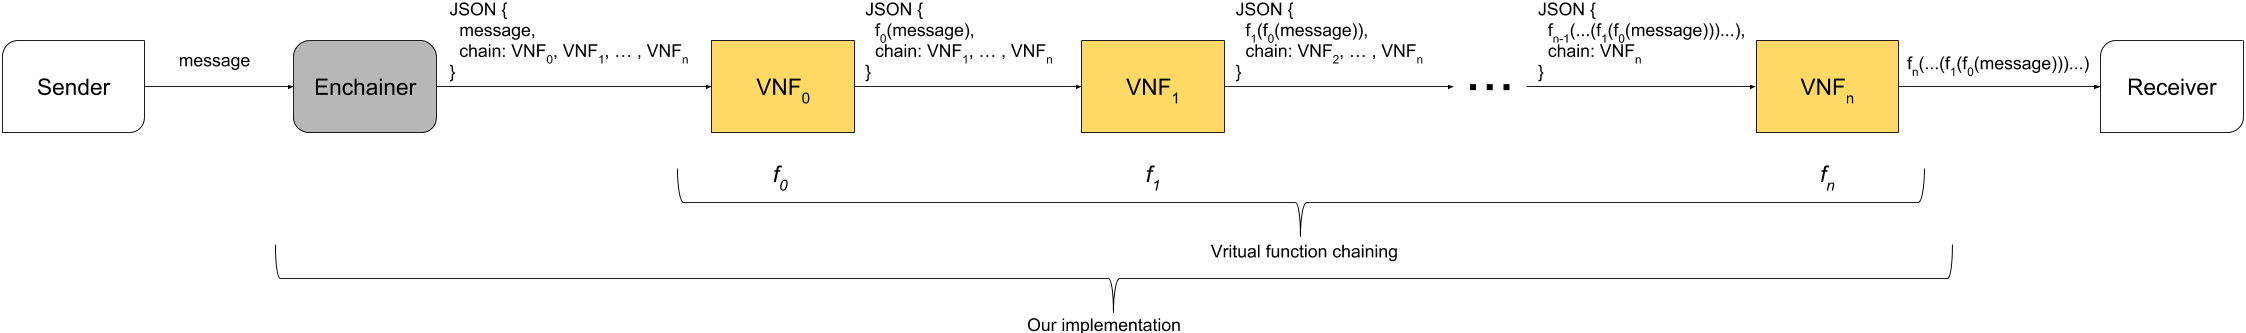
\includegraphics[width=\textwidth]{firstreview}
  \caption{First review schema}
  \label{chap:impl:img:firstreview}
\end{figure}
First SFC implementation was only developed to become familiar with
technologies, in particular with Kubernetes. At this stage of the project there
were not implemented yet any sort of automatic chain deployment. Moreover
there were not any mechanism to retrieve chain or function available and the
path that traffic must traverse were statically defined by the classifier at the
chain edge. This first solution schema is described in
Figure~ \ref{chap:impl:img:firstreview}. Two components were identified:
\begin{itemize}
  \item \enchainer
  \item \vnfs
\end{itemize}
The former element represent the first link on each chain. The goal of this
element is to receive packets from the sender and to query the classifier to
retrieve the SFC composition. After it wraps the message into a JSON file,
along with the path chain specification:
\begin{lstlisting}[language=json]
{
    "message" : "<the original message>",
    "chain": ["<IP vnf1>", "<IP vnf2>", ..., "destination"]
}
\end{lstlisting}
The \texttt{message} field is the original message sent to the chain,
instead the \texttt{chain} field is an array of IPs or Kubernetes service names
that allows to reach VNF. The array even specify VNFs order. The last element
must be the final destination of the packet. 
The \vnf{} in this review are seen as two layer application. One layer is
the ``real'' VNF, so the treatment of the traffic, the other, instead, manage the
communication in the chain. It must provide the capability to
forward packets following this schema:
\begin{enumerate}
  \item once a packet arrives the field \texttt{message} must be read and the
  function represented by the VNF applied;
  \item the field \texttt{chain} must be read and based its values there are two
  possibilities:
  \begin{enumerate}
    \item if array length is greater then $1$ the JSON that wraps the message
    must be reconstructed because the actual \vnf is not the last
    element of the chain. \texttt{message} field must be set to the result of
    of the function application and the \texttt{chain} field must be updated
    removing the first element of the array;
    \item if array length is equal to $1$, after the application of the
    transformation of the VNF to the value of the \texttt{message} field,
    message must be delivered to destination, without the JSON wrapping:
    \item in other case message must be discarded.
  \end{enumerate}
\end{enumerate}

\subsection{Implementation}
This first code implementation was developed in Java\footnote{And available on
this repository: \\\url{https://github.com/Augugrumi/chaining-functionalities}}
The \enchainer{} component is simply a server implemented using Netty
library\footnote{\url{https://netty.io/}}. The choice of this framework is due
the possibility to serve multiple protocols and for its quick and easy usage. 
The \vnf{} component is defined as follow: an interface define methods
that must be implemented, an abstract class extends the previous interface
implementing the communication layer of the interface as well as it manages the
JSON wrapping/unwrapping. \vnf{} communication take advantage of
Rapidoid\footnote{\url{https://www.rapidoid.org/}} library for packet sending
and receiving, both for simplicity and because it gives the opportunity of
managing a large pool of connection in a rapid way. In this prototype solution
it is possible to replace the \vnf{} component with every element that
provides the same JSON wrapping management logic and that gives is capable
to send and receive packets. Java code could be implemented with the different
VNF but alternative implementations (even developed in different languages) are
allowed. 

\subsection{Kubernetes Deployment}
Two alternative approaches where implemented to deploy chain exploiting this
solution: using a single Pod or multiple Pods. First solution, although easier
to deploy is not scalable: all the components of the SFC will run on the same
Kubernetes Node. Second approach make use of different Pods.

\subsubsection*{Single Pod}
To deploy the first review solution using a single Pod the SFC composition is
defined using a single Kubernetes Deployment (in which all the \vnf{} and
the \enchainer{} are specified) and a single Service that exposes the
\enchainer{} and makes it reachable outside the Pod using the Service name.

\subsubsection*{Multiple Pods}
Multiple Pods first review follow a different approach. For each \vnf{}
and for the \enchainer{} is defined a different Deployment and a Service.
Even if it is more cumbersome to define chain like this it helps to create a
more scalable and flexible solution. In fact, exposing each \vnf{} with a
Service allows the single \vnf{} to be part of different SFC and to do not
have static chain created at deployment time. Moreover, handling separately
the components make possible to increase/decrease the number of single
\vnfs{} or of the \enchainer{} basing on traffic load.

\subsection{Problems}
This first attempt has different issues. First \enchainer{} has no
possibility to retrieve all the original message of a sender: it requires at
least that even the transport layer headers can be read, but it is not possible
due to i) server created with Netty works at application layers and ii) Java
does not allow to create socket at an enough low layer that allow transport
layer header reading. To mitigate this and deploy the solution the workaround
was to add to the payload of the message sent the missing headers. Lower layer
header allows the classifier to know more information on the communication, so
to perform a better analysis on the treatment to apply on the incoming packets.
Another problem was the JSON wrapping: it does not follow the standard
encapsulation defined for this technology. Passing to a standard encapsulation
was planned, but the JSON one was useful because of the format, that can be easy
read and write. Further, even the communication among VNF works at application
level using POST request to sends data and lower layer communication can enhance
performance. Finally, with this implementation data sent from the sender must be
fully received to the \enchainer{} before, then from each \vnf{} in
the chain, making communication slower and making it not suitable in some
context such as transfer of heavy files.

\section{Second review}
\begin{figure}
  \centering
  \includegraphics[scale=0.2]{secondreview}
  \caption{Second review schema}
  \label{chap:impl:img:secondreview}
\end{figure}
The second review is an enhancing of the first proposal in which components
organization is changed, as depicted in Figure~\ref{chap:impl:img:secondreview}.
Main goal of this review were to further study technologies involved into the
project and to examine a different approach.

Simultaneously of the development of this proposal we started the development of
the instrumentation that automatize the chain deployment.

In this second proposal three components are defined:
\begin{itemize}
  \item \enchainer{}
  \item \dispatcher{}
  \item \vnfs{}
\end{itemize}
\enchainer{} is pretty the same of the first implementation. Even in this case
the this component must be the first element to be traversed of the chain, that
wrap the message into a JSON format as in the previous solution and define the
list of function that traffic must traverse. \vnfs{}, instead, were revisited.
During the development of this second implementation we thought that they must
be decoupled to the mechanism on encapsulation, leaving to \vnf{} only the task
to perform the function to transform traffic and to implement basic
communication functionalities, as receive a packet and give back a response. The
new element introduced was the \dispatcher{}. It was a centralized component
whose aim is to manage the chain composition and work in this manner: it receive
the JSON wrapped message from the \enchainer{} and retrieve both
\texttt{message} and \texttt{chain} fields values. After it sends the former
value to the first element of the array described from the \texttt{chain} field.
Following this idea, \vnfs{} does not need to know anything about the JSON
formatting (\emph{SFC unaware}) but it only to be able to receive packet on a
certain port, (eventually) modify it and send it back. Basically, the different
approach compared to the previous implementation depends on the presence of the
dispatcher that is accountable of the traffic forwarding.

\subsection{Implementation}
Even this second implementation experiment was developed in Java\footnote{And
available on this repository: \\
\url{https://github.com/Augugrumi/alternative-chaining-functionalities}}. The
\enchainer{} implementation basically was not changed. To the \vnf{} component
was removed the JSON encapsulation code: as in the previous review a hierarchy is
provided, but this time is only need for a more rapid function development. Even
this prototype allow to create \vnf{} using different code or programming
languages, only requirements are:
\begin{itemize}
  \item to be able to receive a POST request;
  \item to be able to modify the payload of the POST request, applying the
  function for which it was created;
  \item to be able to reply to the previous request, sending the modified data.
\end{itemize}
The code managing wrapping is moved to the \dispatcher{}, that make use of
Rapidoid library for ingoing and outgoing communications.

\subsection{Kubernetes Deployment}
Even for this implementation we provide two different deployments, one that
deploy all the system in a single Pod and the other that exploit the possibility
to use multiple Pods. The deployments works as before. In the Single Pod one the
SFC, the \enchainer{} and the \dispatcher{} are specified onto the same
Deployments and a Service is specified to be able to reach the chain. In the
Multiple Pods deployment, as before, each component is defined by a different
Deployment and exposed by a Service.

\subsection{Problems}
This second review, since it is based on the code of the previous one, does not
solve the problems explained before, as the problem regarding application
level communications, the usage of Java as programming language and JSON
wrapping issues. This solution was developed to study a different topology
approach, using a centralize element, the \dispatcher{}, that can be the traffic
orchestrator and can redirect traffic to the \vnfs{}. Also, improving its
capabilities, it could have more information on transformation that packets must
pass through and eventually, reclassify the traffic querying the classifier.
Moreover it provides a total decoupling between SFC platform and network
function that must be applied. Thus, there is the drawback of the centralized
approach. This limit the overall scalability since all function must talk to the
same component. Exploiting Kubernetes functionalities it is possible to augment
replicas of the \dispatcher{}, even automatically. Nevertheless, this approach
seems to be not suitable for large traffic loads and it could be a bottleneck
of the platform.

\section{Final proposal}
\section{Classification}
One o the killing feature of the SFC platform is the capability to classify
traffic based on its typology. In fact, this make the system able to redirect
traffic load on the more appropriate chain of network function and, if needed,
to change the treatment during SFC traverse. Nevertheless, in this
implementation we does not take into account the development of a fully featured
classifier because it is outer of the scope of this project. Nonetheless the
latter element is considered in the overall system functioning but is
implemented only as a mock component: based on the protocol type used on
transport layer used to transmit traffic to the SFC edge, it gives back a
chain identifier. Even in the final proposal only TCP and UDP protocol are
considered.
\subsection{Ingresses end egresses}
\subsection{Astaire}
\subsection{Chain management}
\subsection{Proxies}

\subsection{Kubernetes deployment}

\section{Implementation problems}